\documentclass[11pt,a4paper]{article}
\usepackage[utf8]{inputenc}
\usepackage[T1]{fontenc}
\usepackage[english]{babel}

\title{
	Computer Exercise 1\\
	EL2520 Control Theory and Practice
}
\author{
	Sifan Jiang\\
	sifanj@kth.se\\
	961220-8232
	\and
	Jiaqi Li\\
	jiaqli@kth.se\\
	960326-1711
}

\newcommand{\image}[3]{
	\begin{figure}[!ht]
		\centering
	    \includegraphics[width=#1\textwidth]{#2}
		\caption{#3}
		\label{fig:#2}
	\end{figure}
}

% My packages
\usepackage{algorithm, algorithmic, listings} % Code
\usepackage{amsmath, amstext, amssymb, amsfonts, amsthm, dsfont, cancel, gensymb, mathtools, textcomp} % Math
\usepackage{color, xcolor} % Color
\usepackage{diagbox, tabularx} % Table
\usepackage{enumerate} % List
\usepackage{epsfig, epstopdf, graphicx, multicol, multirow, palatino, pgfplots, subcaption, tikz} % Image.
\usepackage{fancybox}
\usepackage{verbatim}


\usepackage[font=footnotesize]{caption} % labelfont=bf
\usepackage[font=scriptsize]{subcaption} % labelfont=bf
\usepackage[margin=1in]{geometry}
\usepackage[hidelinks]{hyperref}
\epstopdfsetup{outdir=./Figure/Converted/}
\graphicspath{{./Figure/}}

\makeatletter
\def\input@path{{./Figure/}}
\makeatother

\pgfplotsset{compat=1.13}

\begin{document}
\maketitle

% Minimum phase case
\section*{Minimum phase case}
\par The controller is given by
\begin{align*}
	F(s) = \begin{bmatrix}
		1.6776(1+\dfrac{1}{5.904s}) & 0 \\
		0 & 2.0137(1+\dfrac{1}{6.391s})
	\end{bmatrix}		
\end{align*}
\begin{figure}[!ht]
	\footnotesize
	\centering 
	\begin{subfigure}[t]{.495\linewidth}
		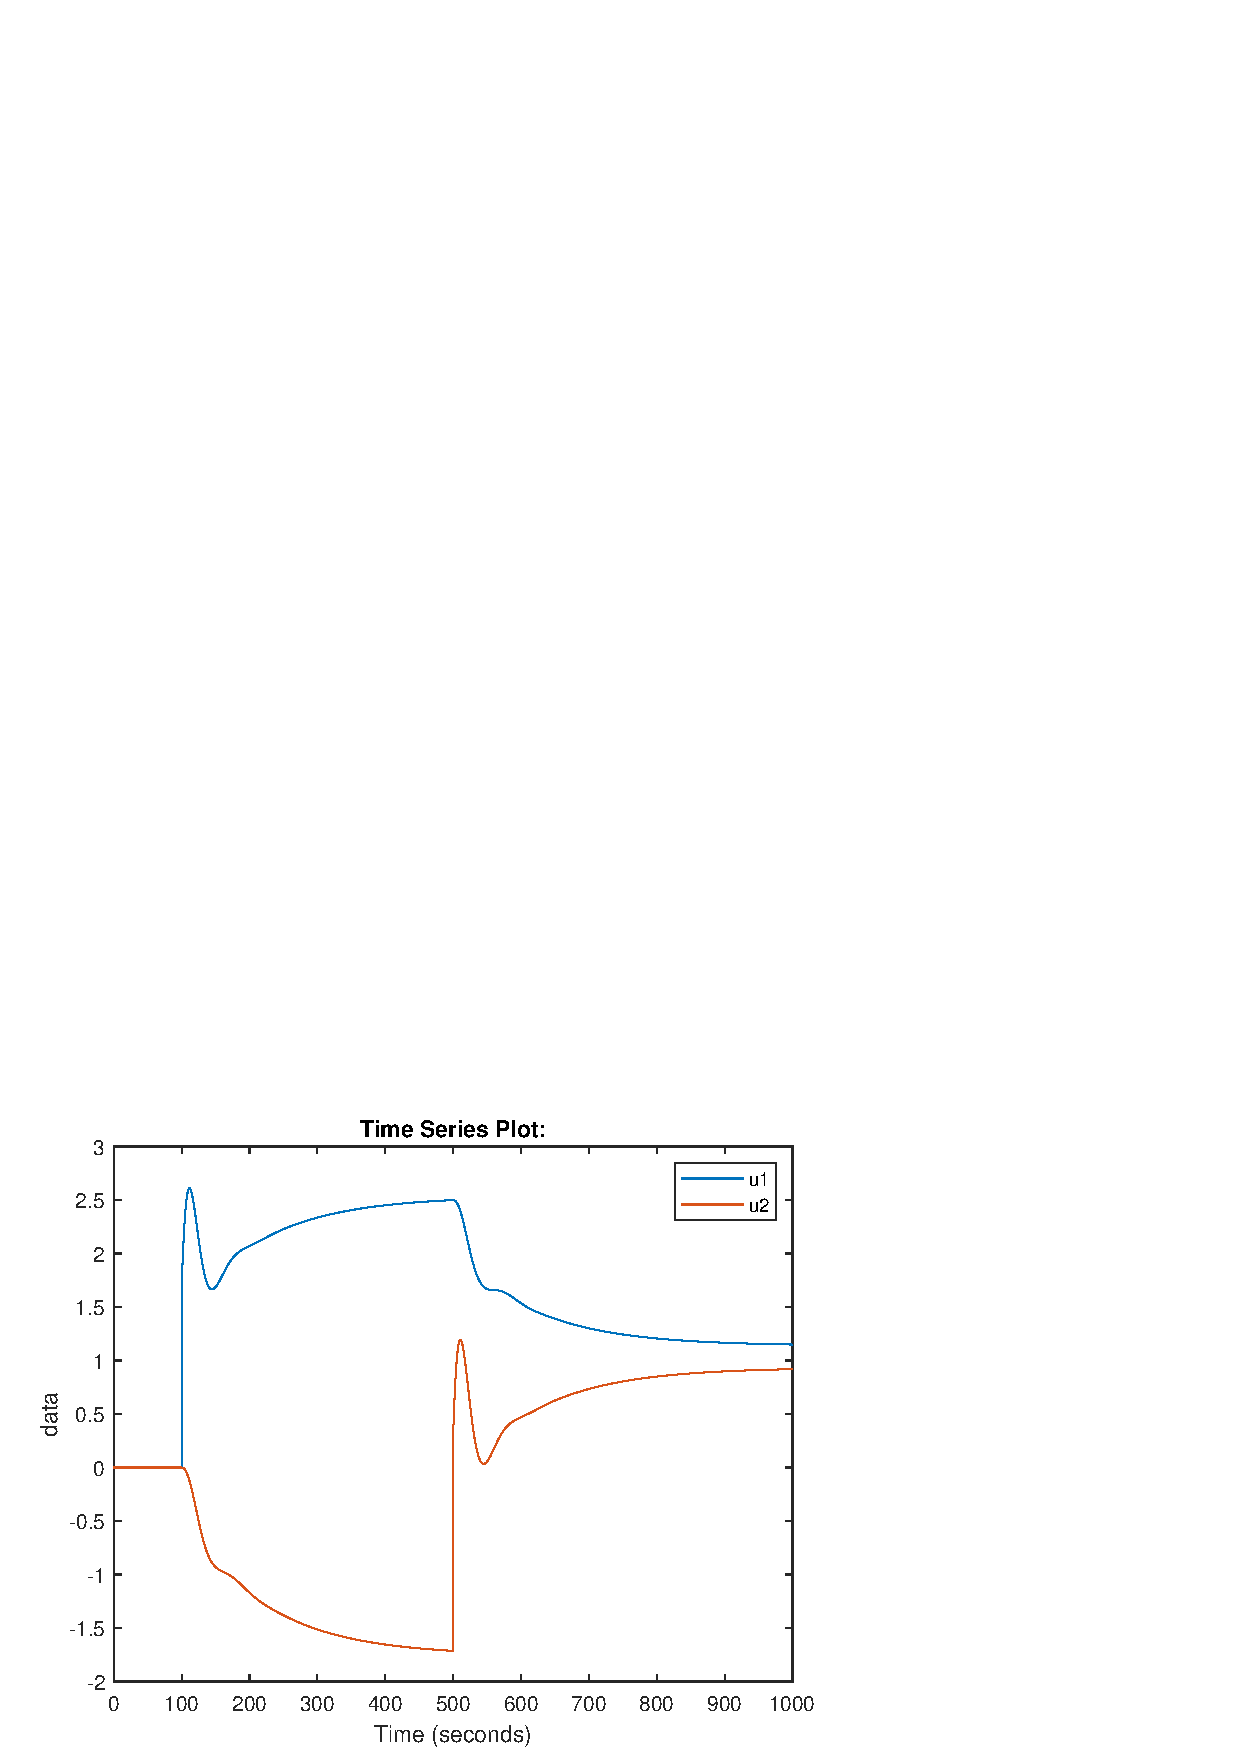
\includegraphics[width=\columnwidth]{3231}
		\caption{Response of the control signal $u$.}
		\label{fig:3231}
	\end{subfigure}
	\begin{subfigure}[t]{.495\linewidth}
		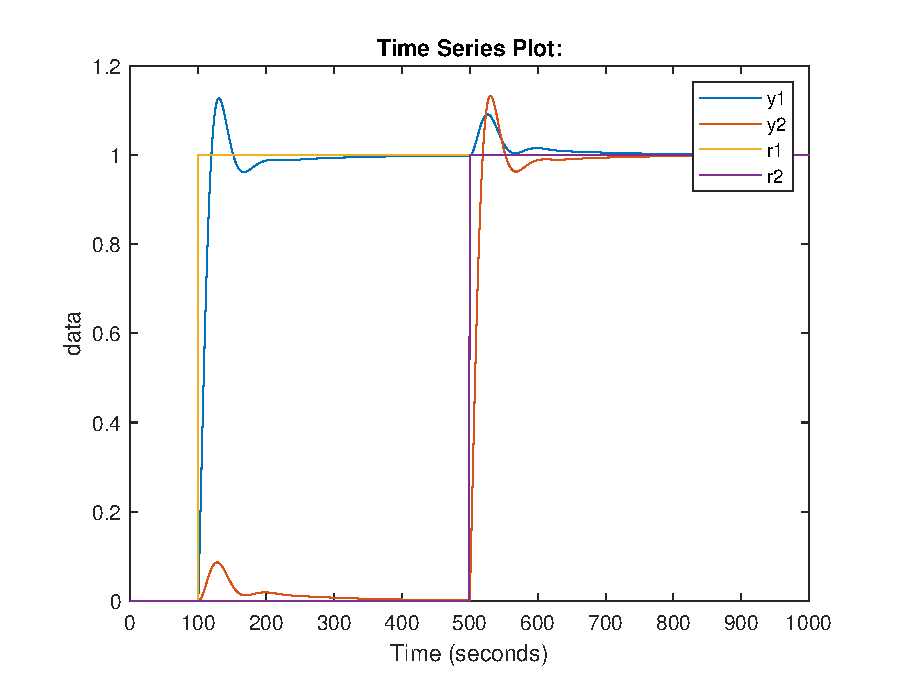
\includegraphics[width=\columnwidth]{3232}
		\caption{Response of the output $y$ with the reference $r$.}
		\label{fig:3232}
	\end{subfigure}
	\caption{Simulink plots from exercise 3.2.3.}
	\label{fig:MPSimulink}
\end{figure}
\begin{figure}[!ht]
	\footnotesize
	\centering 
	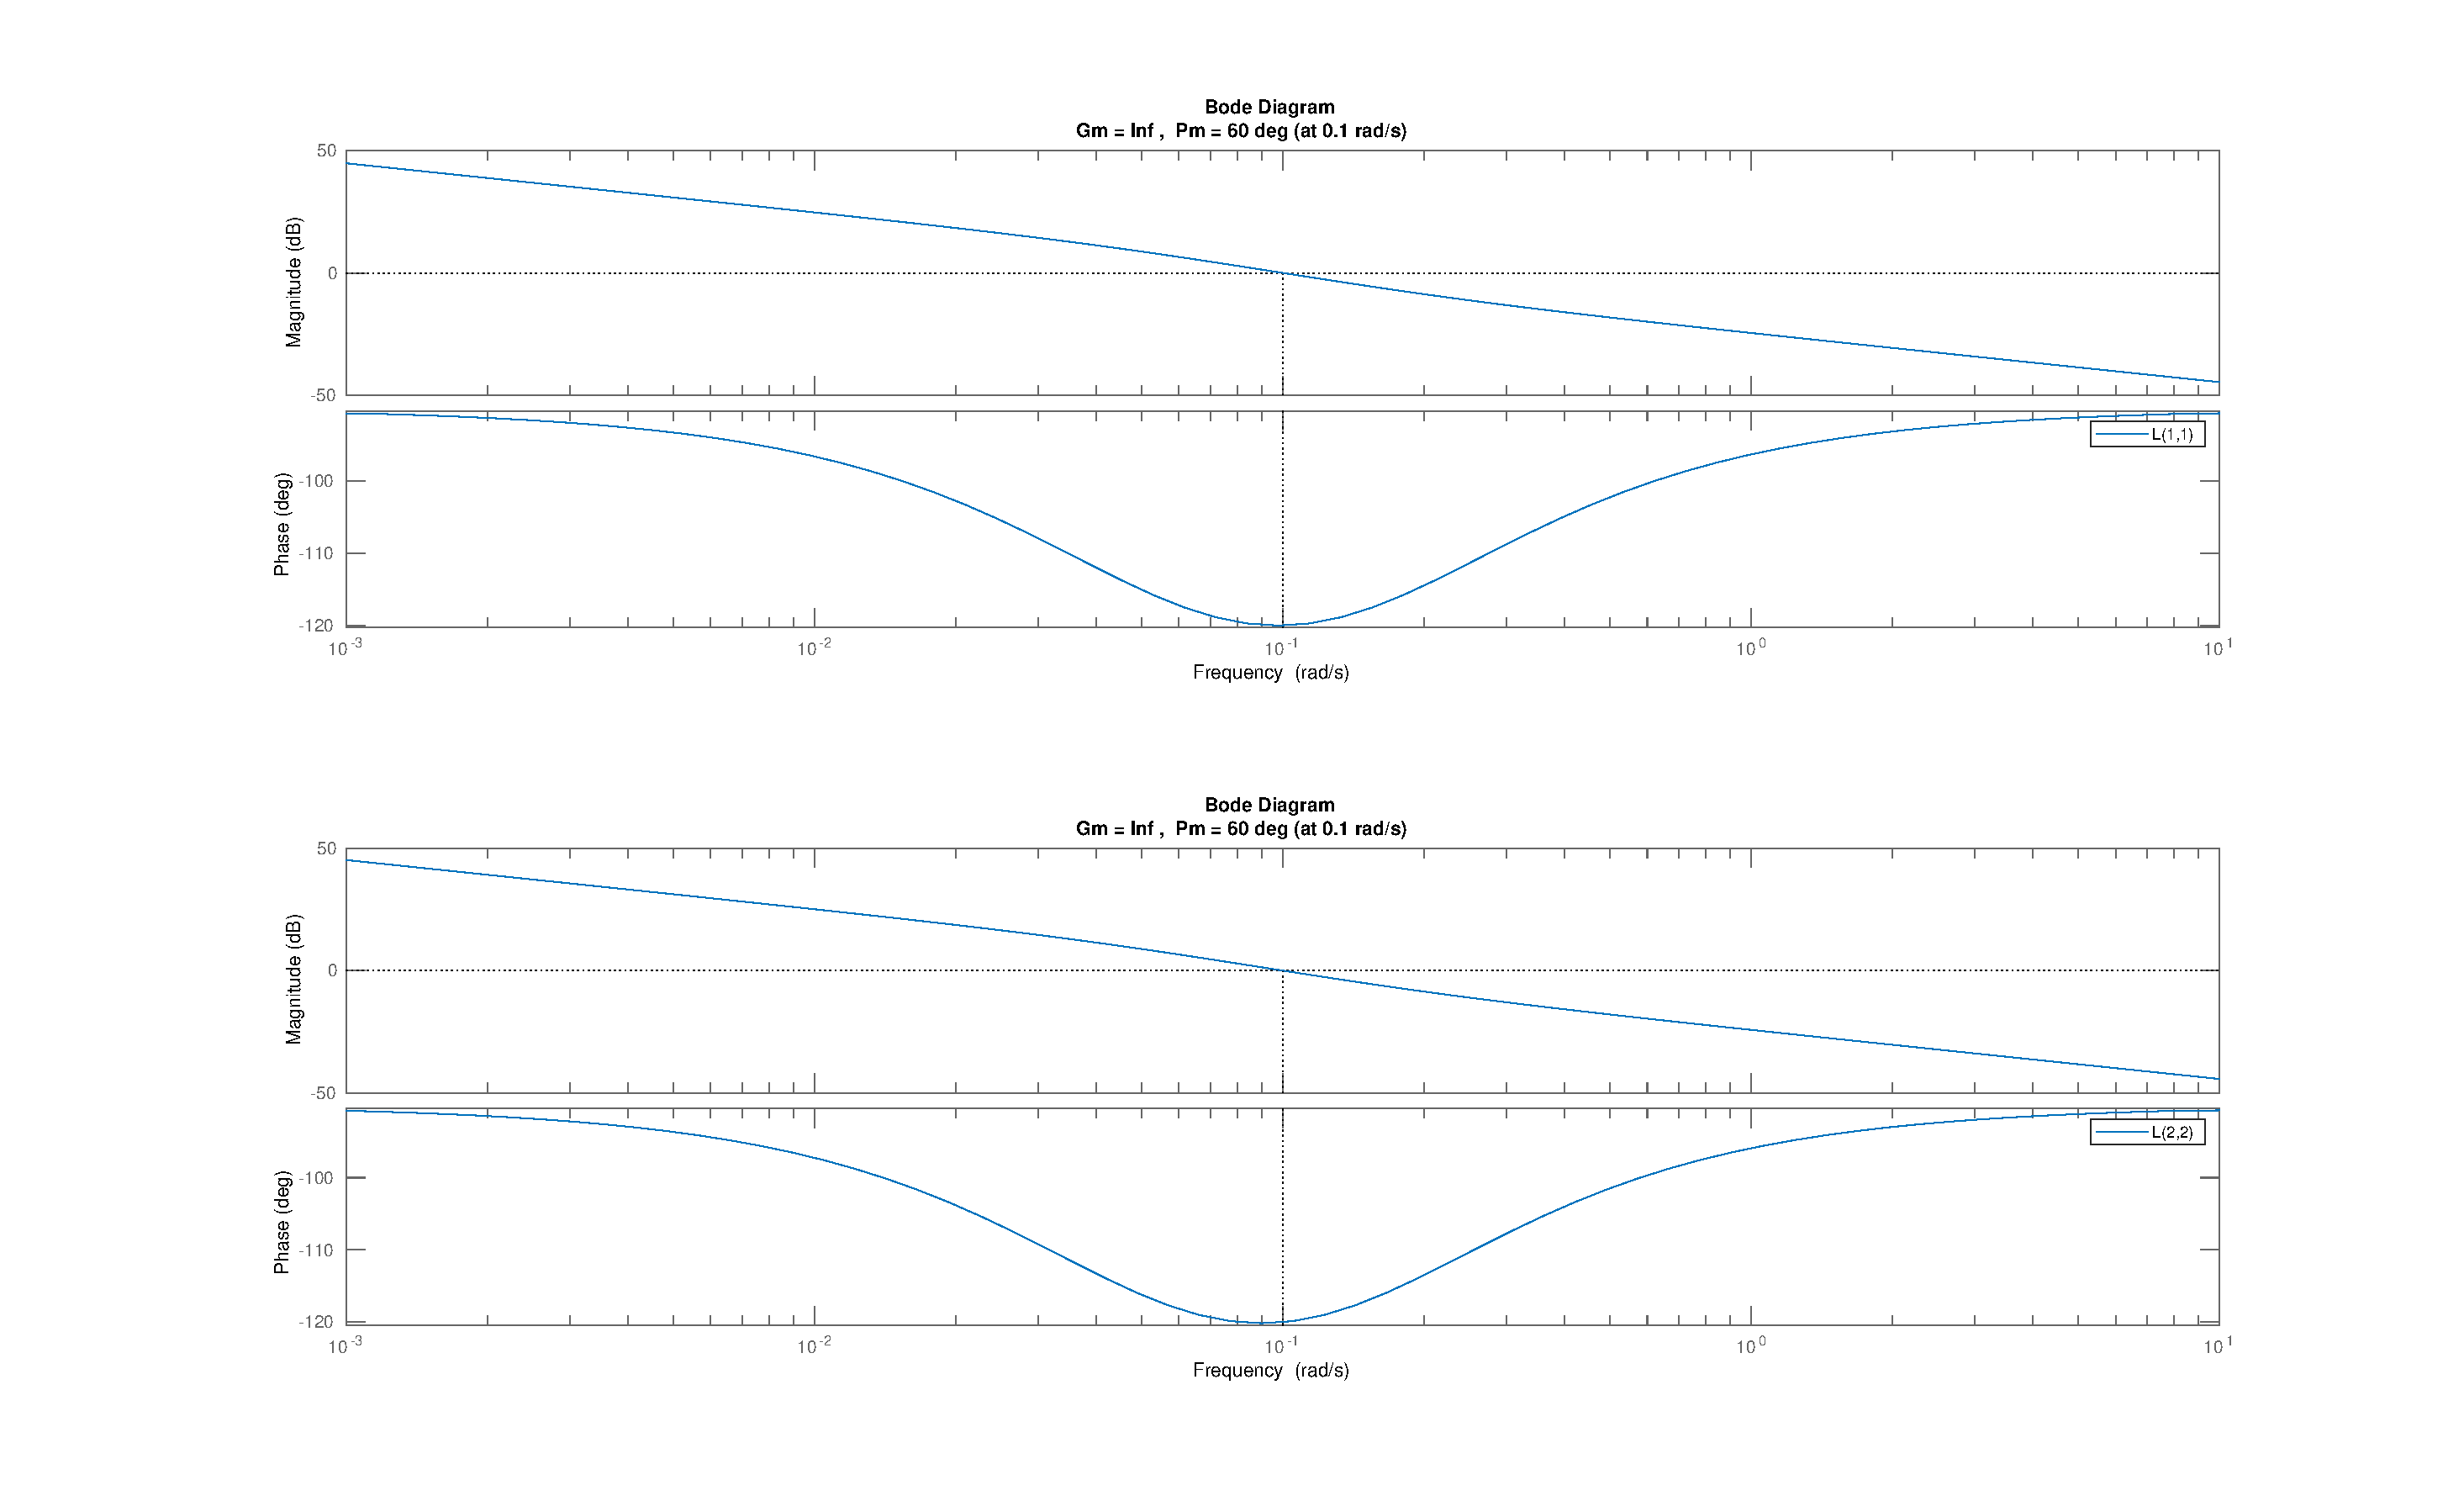
\includegraphics[width=\textwidth]{321}
	\caption{Bode diagram of the loop gain $L(s)$ from exercise 3.2.1.}
	\label{fig:MPBodeL}
\end{figure}
\begin{itemize}
\item Is the controller good?
\par Yes, the controller is good.

\item Are the output signals coupled?
\par Yes, the output signals are coupled.
\end{itemize}


% -------------------------------------------------- %
% Non-minimum phase case
\section*{Non-minimum phase case}
\par The controller is given by
\begin{align*}
	F(s) = \begin{bmatrix}
    	0 & 0.1469(1+\dfrac{1}{3.9426s}) \\
    	0.1437(1+\dfrac{1}{4.8107s}) & 0
    \end{bmatrix}
\end{align*}
\begin{figure}[!ht]
	\footnotesize
	\centering 
	\begin{subfigure}[t]{.495\linewidth}
		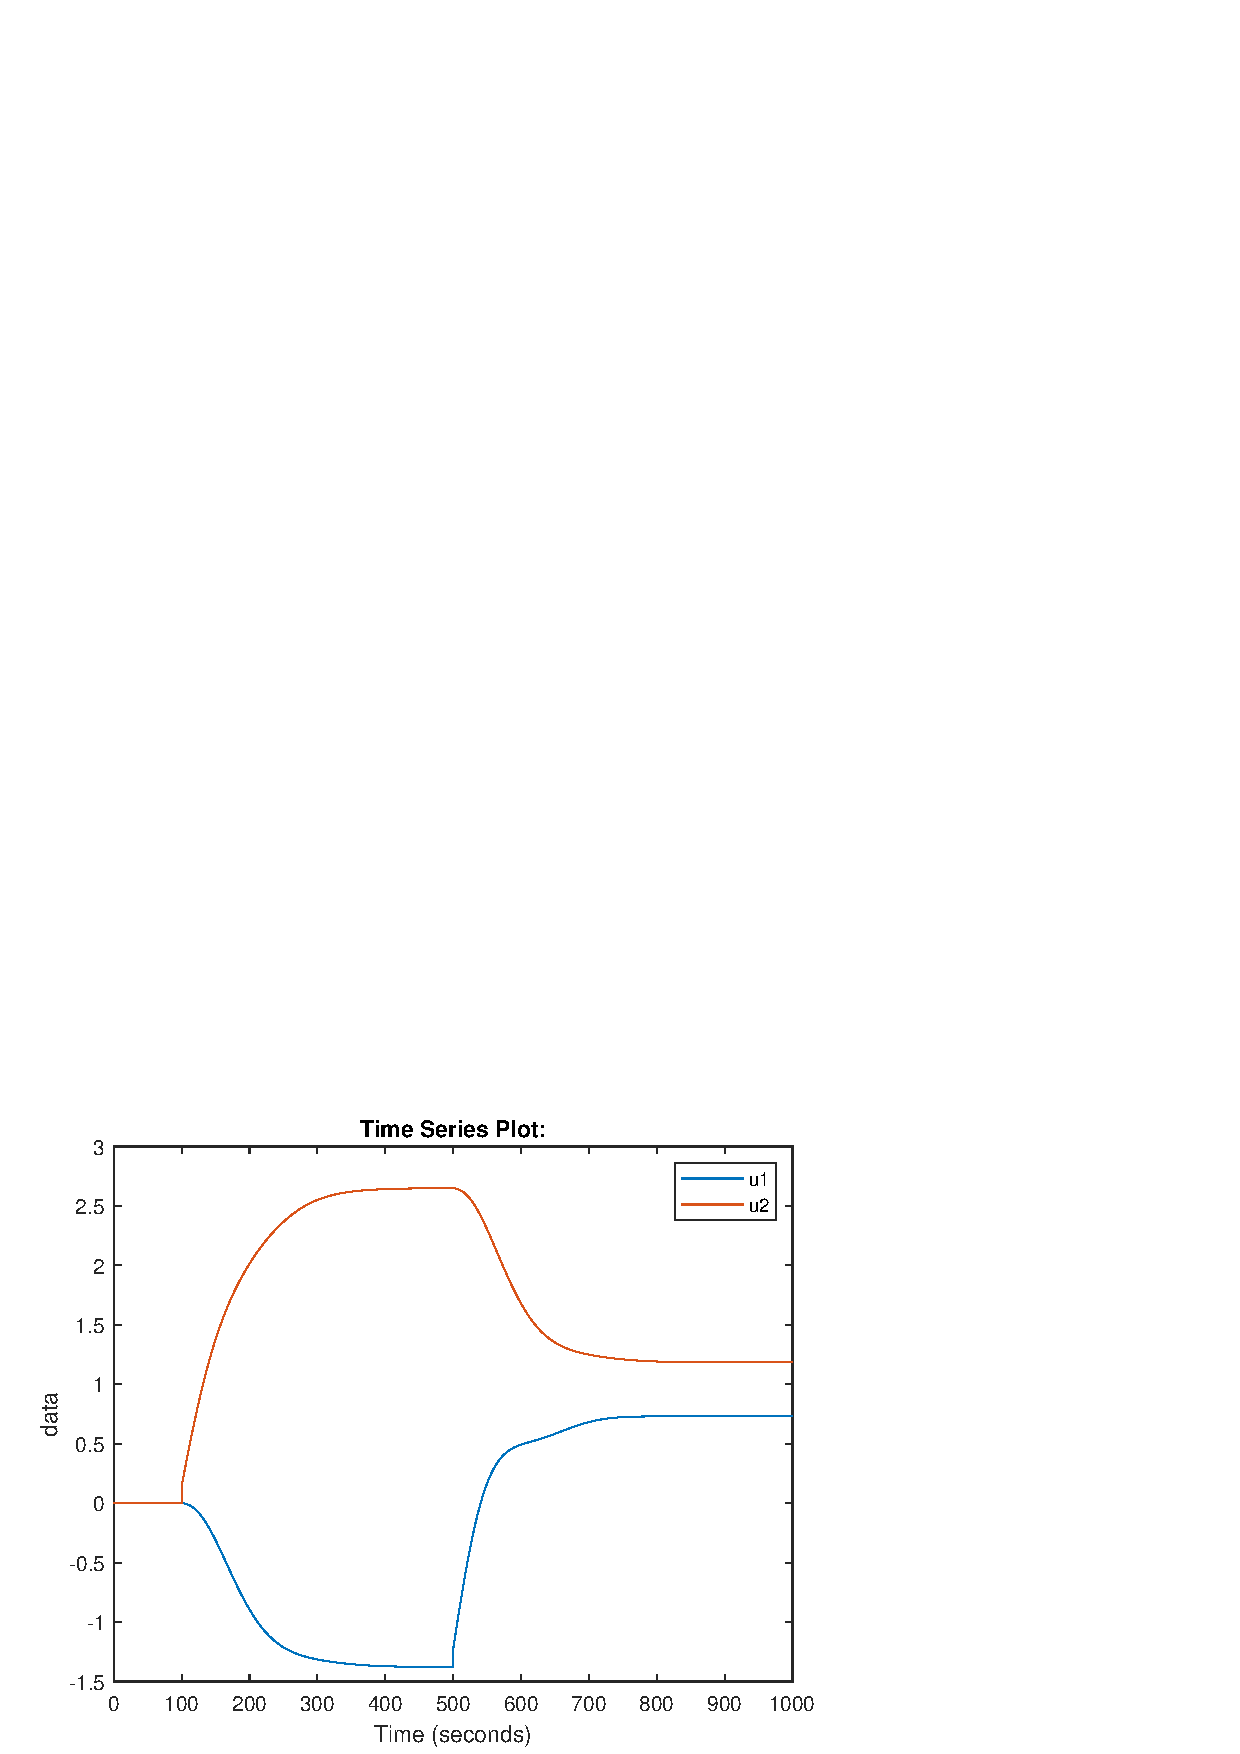
\includegraphics[width=\columnwidth]{3331}
		\caption{Response of the control signal $u$.}
		\label{fig:3331}
	\end{subfigure}
	\begin{subfigure}[t]{.495\linewidth}
		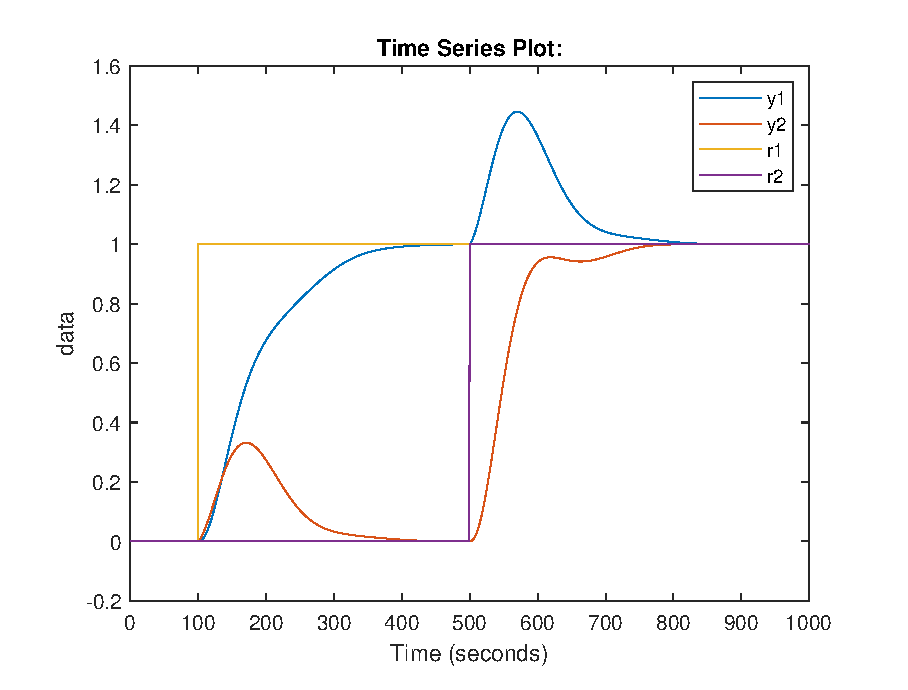
\includegraphics[width=\columnwidth]{3332}
		\caption{Response of the output $y$ with the reference $r$.}
		\label{fig:3332}
	\end{subfigure}
	\caption{Simulink plots from exercise 3.2.3.}
	\label{fig:NMPSimulink}
\end{figure}
\begin{figure}[!ht]
	\footnotesize
	\centering 
	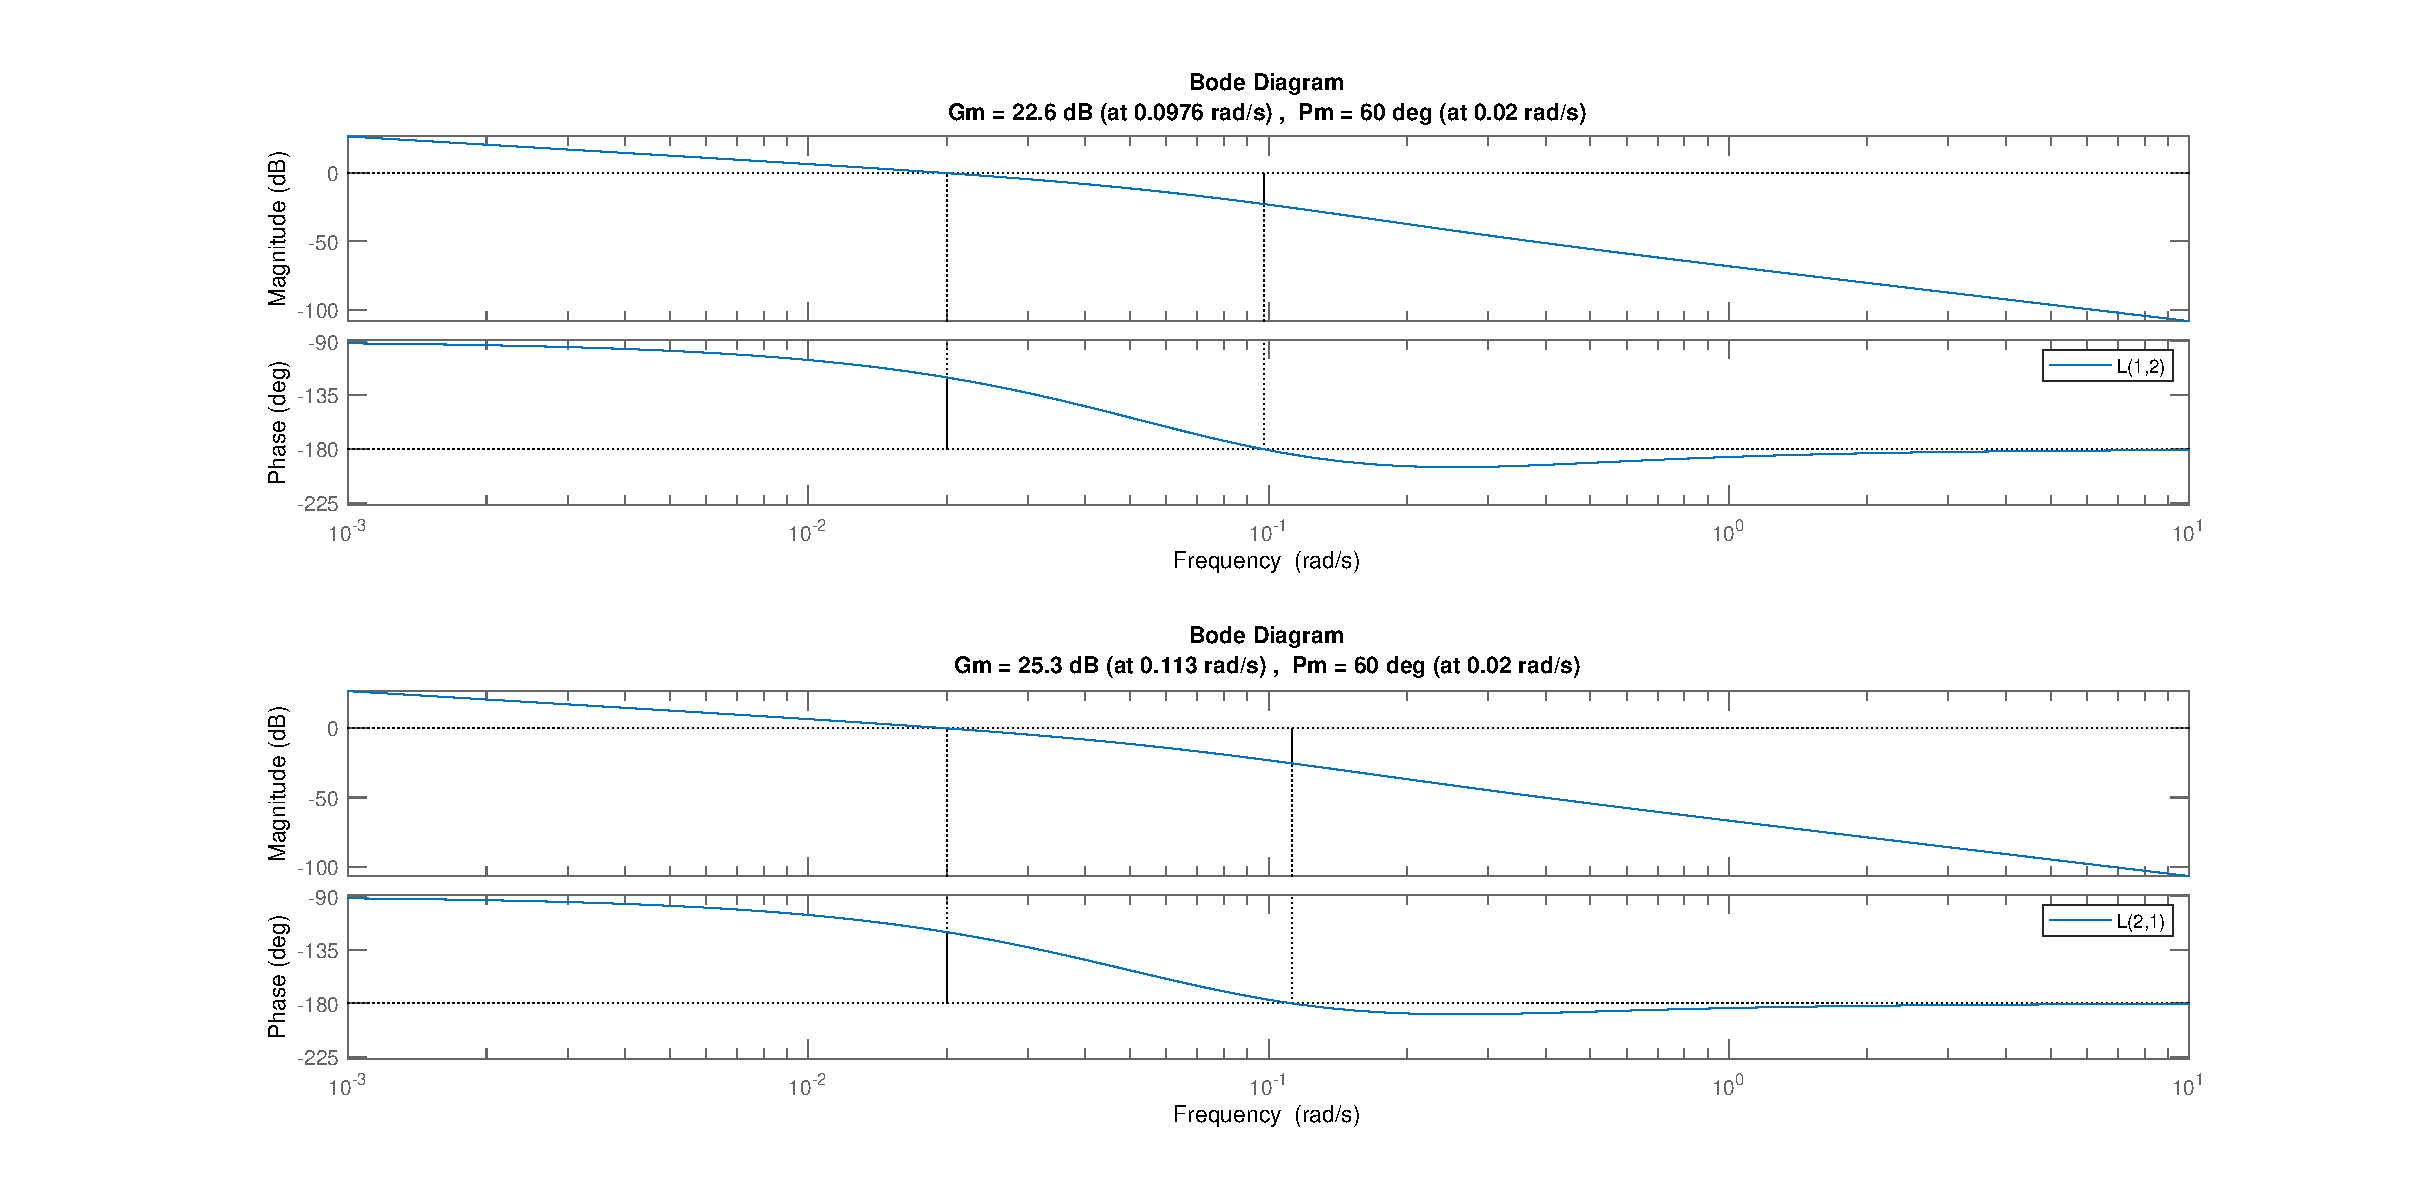
\includegraphics[width=\textwidth]{331}
	\caption{Bode diagram of the loop gain $L(s)$ from exercise 3.2.1.}
	\label{fig:NMPBodeL}
\end{figure}
\begin{itemize}
\item Is the controller good?
\par Yes, the controller is good.

\item Are the output signals coupled?
\par Yes, the output signals are coupled.
\end{itemize}


\end{document}